\documentclass[a4paper]{article}
\usepackage[ruled]{algorithm2e}
\usepackage{fullpage} % Package to use full page
\usepackage{parskip} % Package to tweak paragraph skipping
\usepackage{tikz} % Package for drawing
\usepackage{amsmath}
\usepackage{hyperref}
\usepackage{amsfonts}
\usepackage{float}

\title{Report for Computer Project of Applied Stochastic Analysis---Problem 1}
\author{Liangyu Zhang \\ \\ ID:1500010720}
\linespread{1.5}
\date{December 19, 2018}
\begin{document}

\maketitle

\section{Preliminaries}
\subsection{Ising Model}

The simplest system that exhibits a phase transition is the Ising model. Though in this report the Ising model will be used to model the phase transition of magnetic materials, this model is broadly applicable. Many papers are published each year applying the Ising model to problems in social behavior, neural networks, and other topics. The model was first proposed by Wilhem Lenz. Ising solved the model exactly in one dimension, and in 1944 Lars Onsager solved the Ising model exactly in two dimensions in the absence of an external magnetic field.

Let us consider 2D Ising model, where $N^2$ spins $\sigma=\pm1$ are located in regularly spaced sites of a square lattice $N \times N$. In general, such spins can interact with each other with some coupling energy $J$. Apart from internal interactions within such an ensemble of spins, one could also take into account interactions of each spin with the external magnetic field. And the Hamiltonian $H$ of the system reads:
\begin{displaymath}
H=-J\sum_{\left<i,j\right>}\sigma_i\sigma_j-h\sum_i\sigma_i
\end{displaymath}
, $<i, j>$ means the nearest neighbor interaction, $h$ is the external magnetic strength. Physically the following quantities are of interest:
\begin{itemize}
    \item Internal energy:
        \begin{displaymath}
        U_M=\left<H(\sigma)\right>=\sum_{\sigma} H(\sigma)\frac{e^{-\beta H(\sigma)}}{Z_M}
        \end{displaymath}
    , where $Z_M=\sum_\sigma e^{-\beta H(\sigma)}$. Correspondingly we may define the internal energy per site: $u_M=U_M/N^2$.
    \item Specific heat:
        \begin{displaymath}
        C_M =\frac{\partial UM}{\partial T} =k_B\beta^2\left<H^2(\sigma)\right> - \left <H(\sigma)\right>^2
        \end{displaymath}
    . Correspondingly we may define the specific heat per site: $c_M = C_M/N^2$.
    \item Magnetization:
        \begin{displaymath}
        G_M = \left< \sum_\sigma H(\sigma) \right >
        \end{displaymath}
    . Correspondingly we may define the magnetization per site: $g_M = G_M/N^2$.
    \item Spatial correlation function:
        \begin{displaymath}
        \Gamma(r)=\left<\rho(0)\rho(r)\right>
        \end{displaymath}
    , and the correlation length $\xi$ as the characteristic length that $\Gamma(r)$ decays to 0. Here $\rho(r)$ is the spatial configuration field of $\sigma$. 
\end{itemize}
\subsection{Metropolis Algorithm}
The Standard Metropolis algorithm is a special case of Markov Chain Monte Carlo method. It sets up a Markov chain by defining a suitable proposal matrix $Q$ and a decision rule $A$ correspondingly, such that the probability density of $\frac{1}{Z_M}e^{-\beta H(\sigma)}$ is the only equilibrium of this Markov Chain. And detailed description of the algorithm is shown as follows:\\
\textbf{Algorithm 1.}\textit{(Metropolis Algorithm)}
\begin{itemize}
    \item \textit{Step 1.} Generate the proposal sate $\sigma '$ from state $\sigma_t$  according to the proposal matrix, namely, we have $P(\sigma'|\sigma_t)=Q(\sigma_t\to \sigma ')$;
    \item \textit{Step 2.} Define $\Delta H=H(\sigma') - H(\sigma_t)$, compute
    \begin{displaymath}
    A(\sigma_t\to\sigma')= \begin{cases} 
    1, &\Delta H < 0\\
    e^{-\beta \Delta H}, &\Delta H \geq 0
    \end{cases}
    \end{displaymath};
    \item \textit{Step 3.} Generate R.V. $r\sim U[0,1]$;
    \item \textit{Step 4.} If $r < A(\sigma_t \to \sigma')$, $\sigma_{t+1}=\sigma'$; else, $\sigma_{t+1}=\sigma_t$. Then set $t \gets t+1$, turn to Step1.
\end{itemize}
Therefore, according to the Ergodic theorem, we may approximate the ensemble average by the time average, namely:
\begin{displaymath}
\left< f(\sigma) \right> \approx \sum_{t=1}^T f(\sigma_t)
\end{displaymath}.

\section{Detailed Solutions}
\subsection{Solution for part a)}
In part a) we would like to compute the internal energy per site and the specific heat per site of the system at different temperatures via the Metropolis method and thus identify the critical temperature $T^*$ of the phase transition. Here we set the size of the system $N$ to be $50$, the coupling energy $J$ to be $1$ and the external magnetic strength $h$ to be $0$. The proposal rule $Q$ is set to be:
\begin{displaymath}
Q(\sigma \to \sigma')=\begin{cases}
\frac{1}{N^2}, &\sigma\ \text{and}\ \sigma'\ \text{differs at only one site}\\
0, &\text{otherwise}
\end{cases}
\end{displaymath}
, and the initial state $\sigma_0$ is set to be all $+1$, because otherwise our algorithm may not be able to converge to the equilibrium at very low temperatures.

The programming language we use to perform the simulation is C++ and the data processing and visualization step is completed using Python package Numpy and Matplotlib. $T$, the total number of iterations, is chosen as $10^6$, which is believed to be sufficiently large. And the simulation result is shown in the following pictures:

\begin{figure}[ht]
\centering
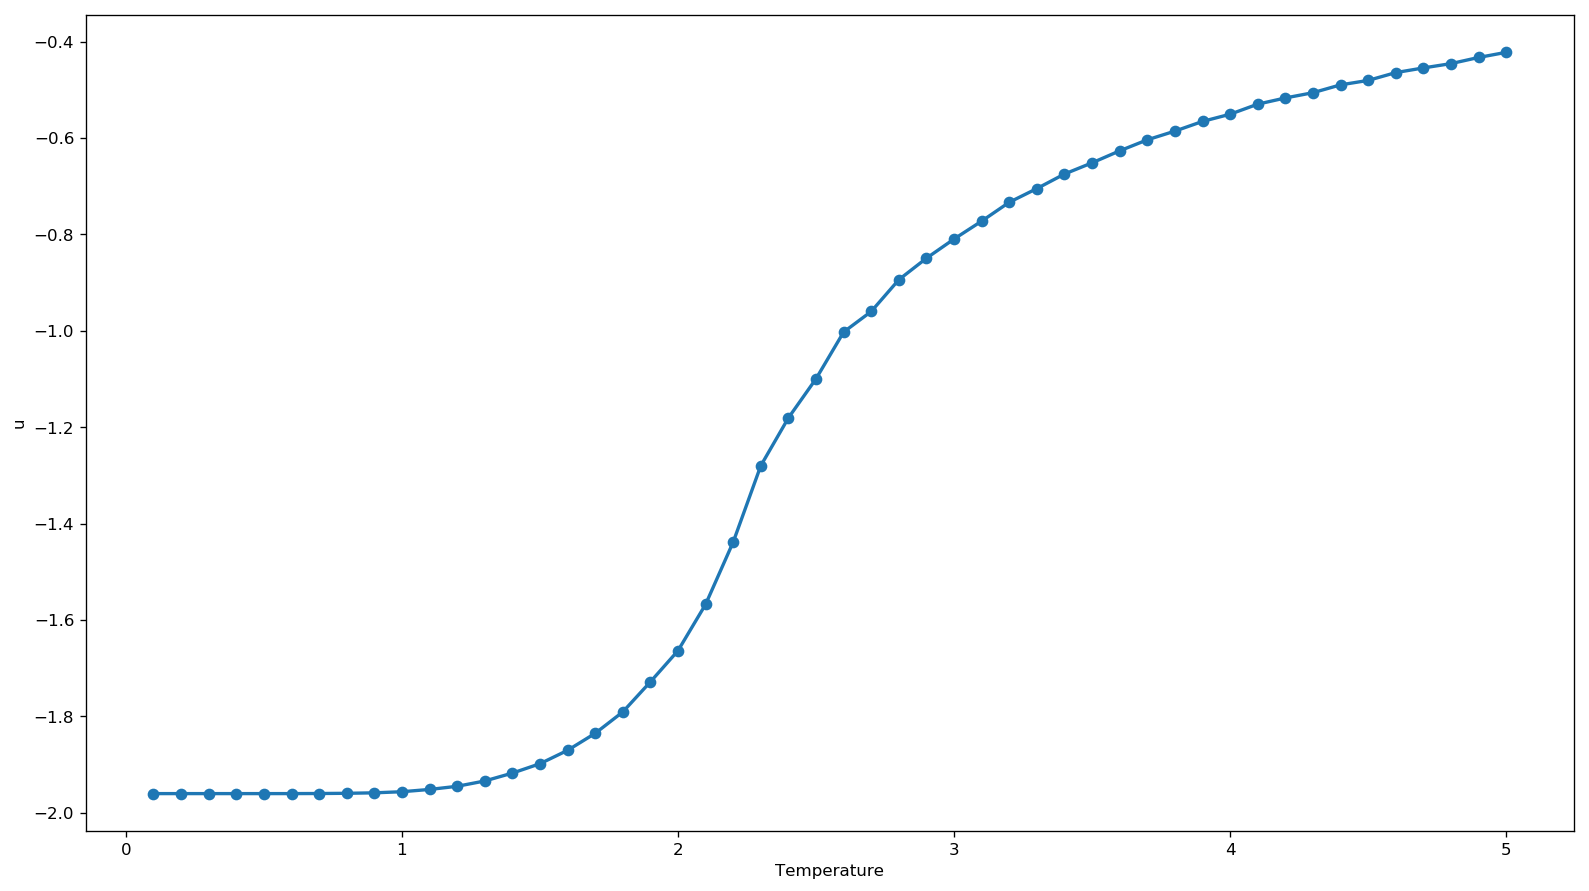
\includegraphics[scale=0.325]{u.png}
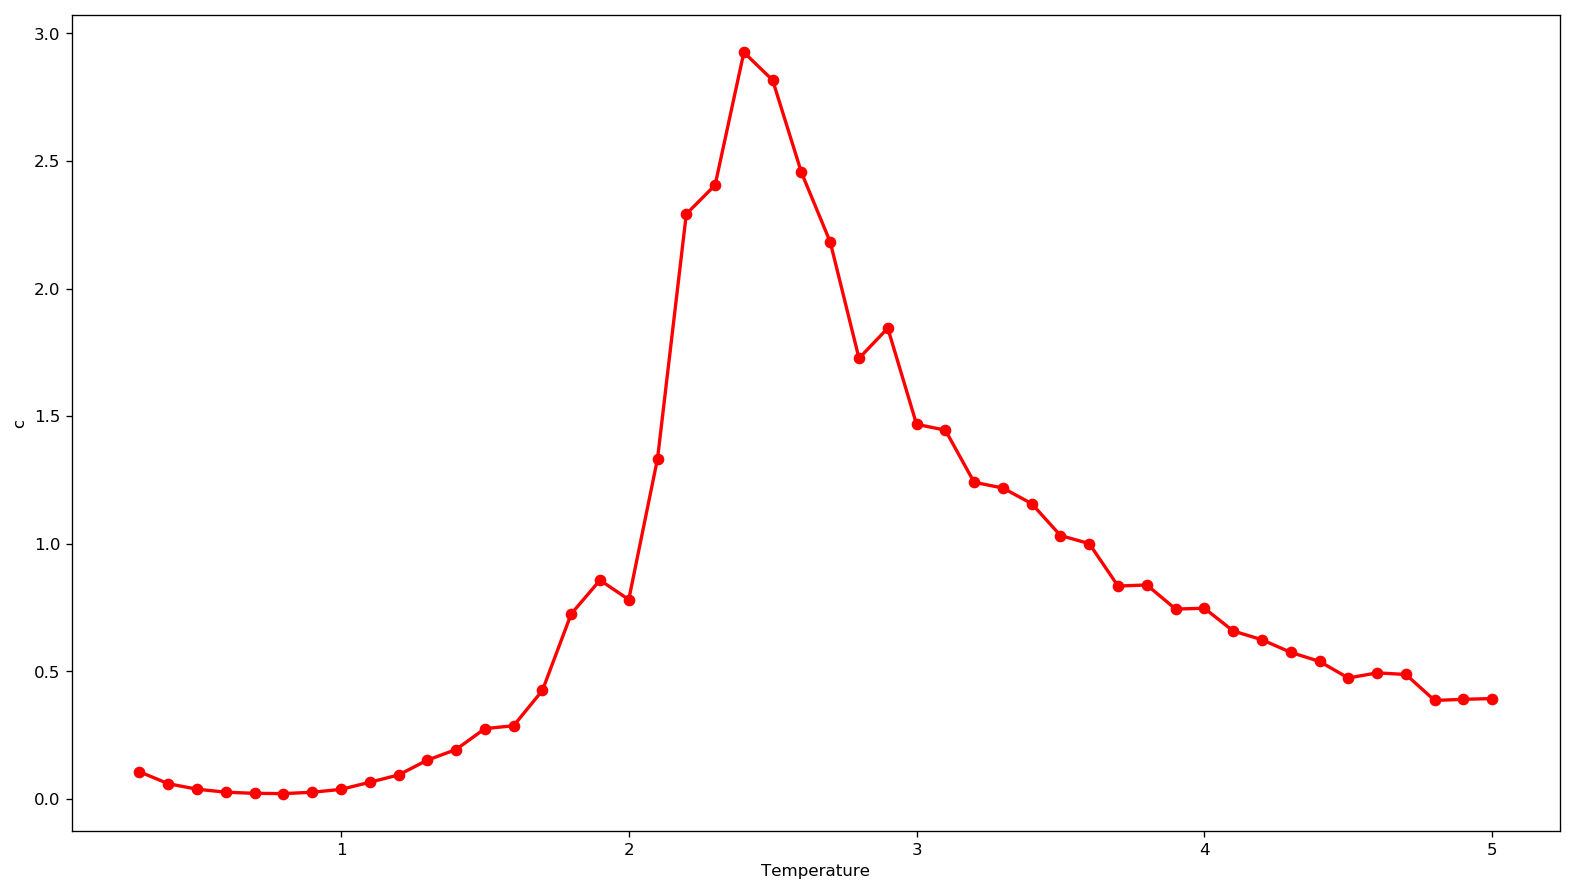
\includegraphics[scale=0.325]{c.png}
\end{figure}


According to the plot above we may easily identify that the critical temperature is in the range $[2.2,2.4]$, which is quite close to the theoretical value $T^*=2/(log(1+\sqrt{2}))\approx 2.269$. 

\subsection{Solution for part b)}
Here we would like to investigate the relationship between the magnetization per site $g_M$ between the the external magnetic strength $h$ at different temperatures. All the settings remain exactly the same as \textbf{section 2.1} except for $h$. And our simulation results are:
\begin{figure}[H]
\centering
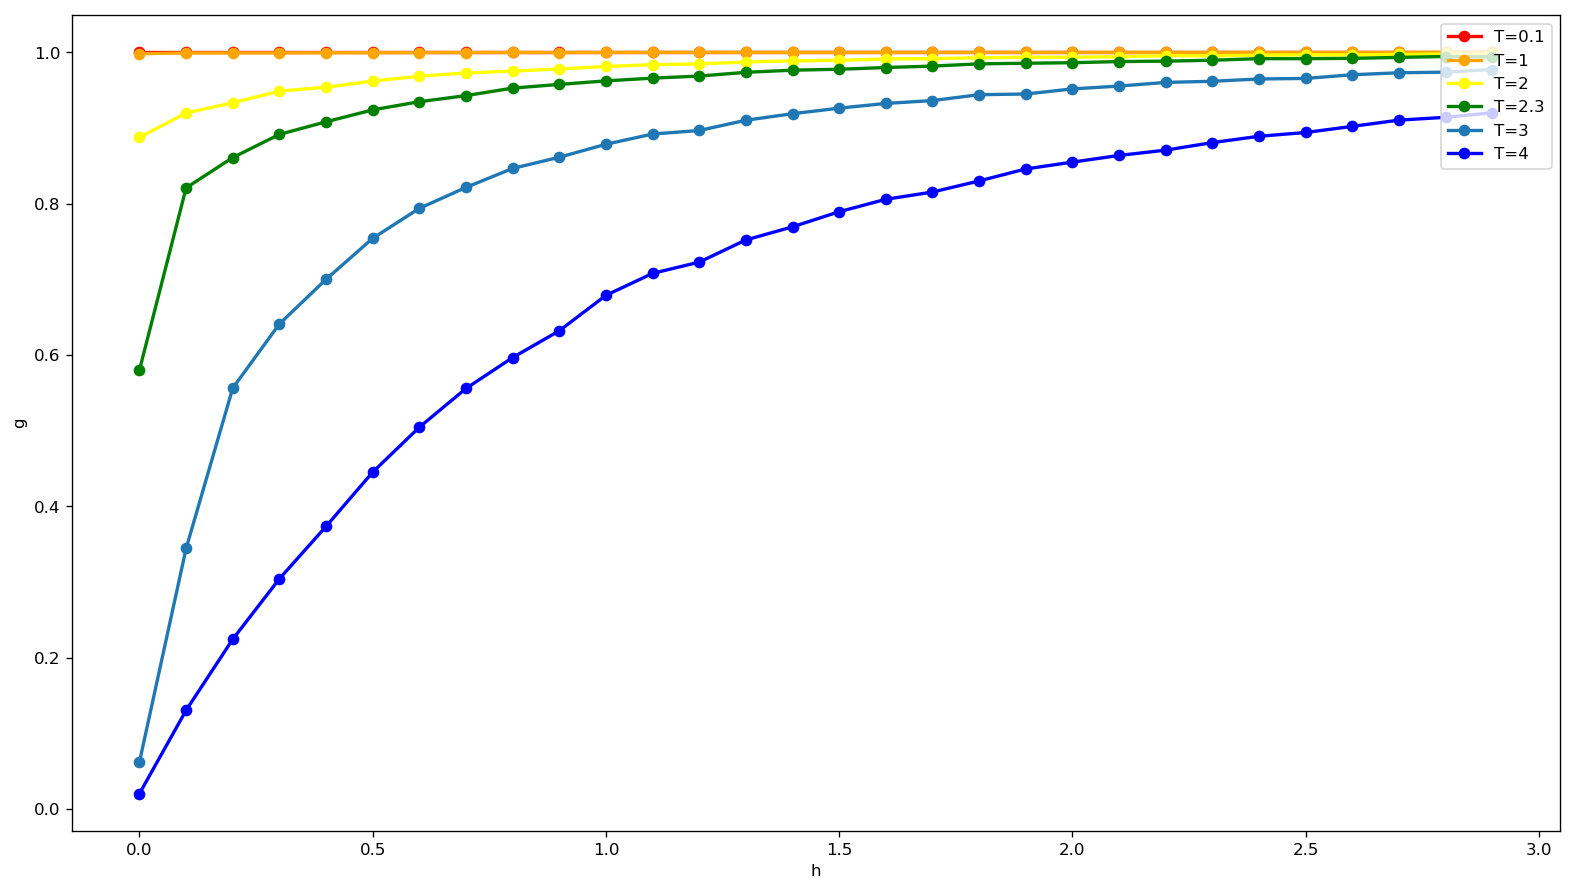
\includegraphics[scale=0.325]{g.png}
\end{figure}
We may notice that when $T<T^*$, $h$ has little impact on $g_M$, but when $T>T^*$ $g_M$ grows gradually to $1$ as $h$ grows. And for larger $T$, $h$ would draw greater influence on $g_M$.

\subsection{Solution for part c)}
In part c) we are to study the correlation length $\xi$ as the function of the temperature $T$. Generally speaking, the correlation length can be considered as a measure of orderliness. As shown in \textbf{section 2.1}, for lower temperatures, the internal energy is also lower. Therefore the system should be more ordered, with large clusters composed of spins with the same directions. Similarly, when the temperature is high, the internal energy is high, too. Thus we would have a system in disorder, and no clear cluster can be observed. Clearly systems in order should have larger correlation length, while disorderly systems are supposed to have smaller correlation length. Just as the following pictures shows:
\begin{figure}[H]
\centering
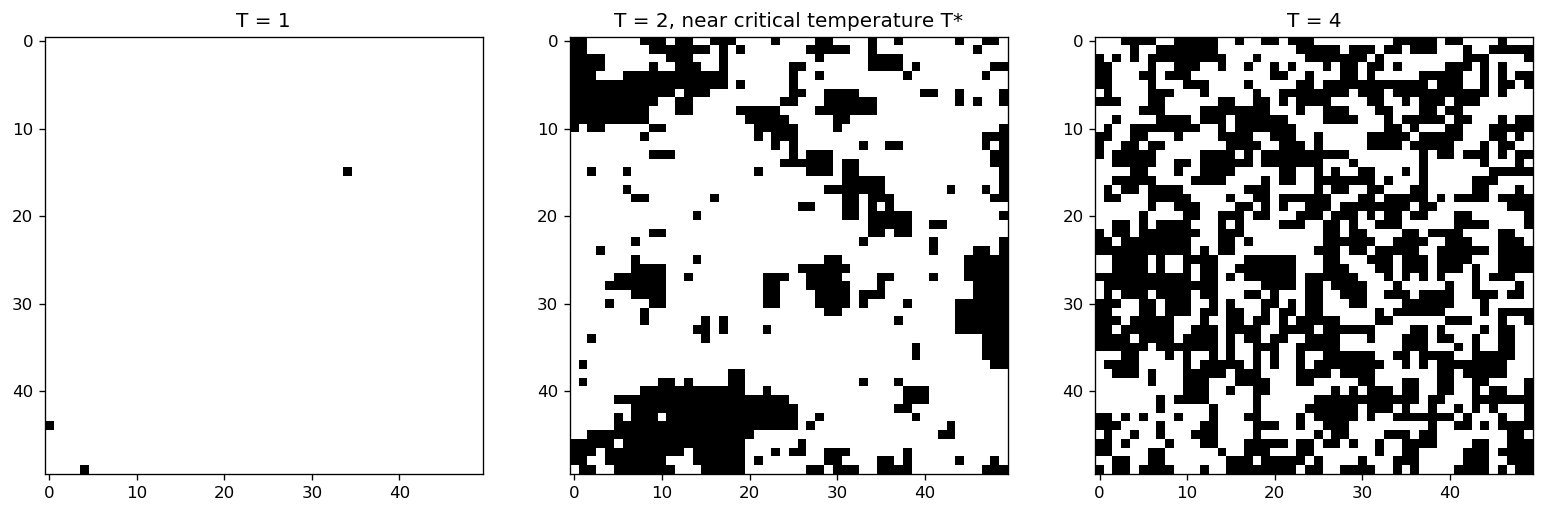
\includegraphics[scale=0.325]{config_visualization.png}
\end{figure}

In our simulation all the settings are the same as in part a), and we approximate $\Gamma(r)$ in the following ways:
\begin{displaymath}
\hat\Gamma(r) = \left<\sigma(i,j)\sigma(i+r,j) \right>
\end{displaymath}
, where $(i,j)$ are randomly chosen satisfying $i \leq N-r$. Clearly the correlation function should decrease monotonically with respect to r. And from theoretical analysis of 2D Ising model we have $\Gamma(r)=e^{-r/\xi}$. Here are our numerical results, which meet our expectation fairly well:
\begin{figure}[H]
\centering
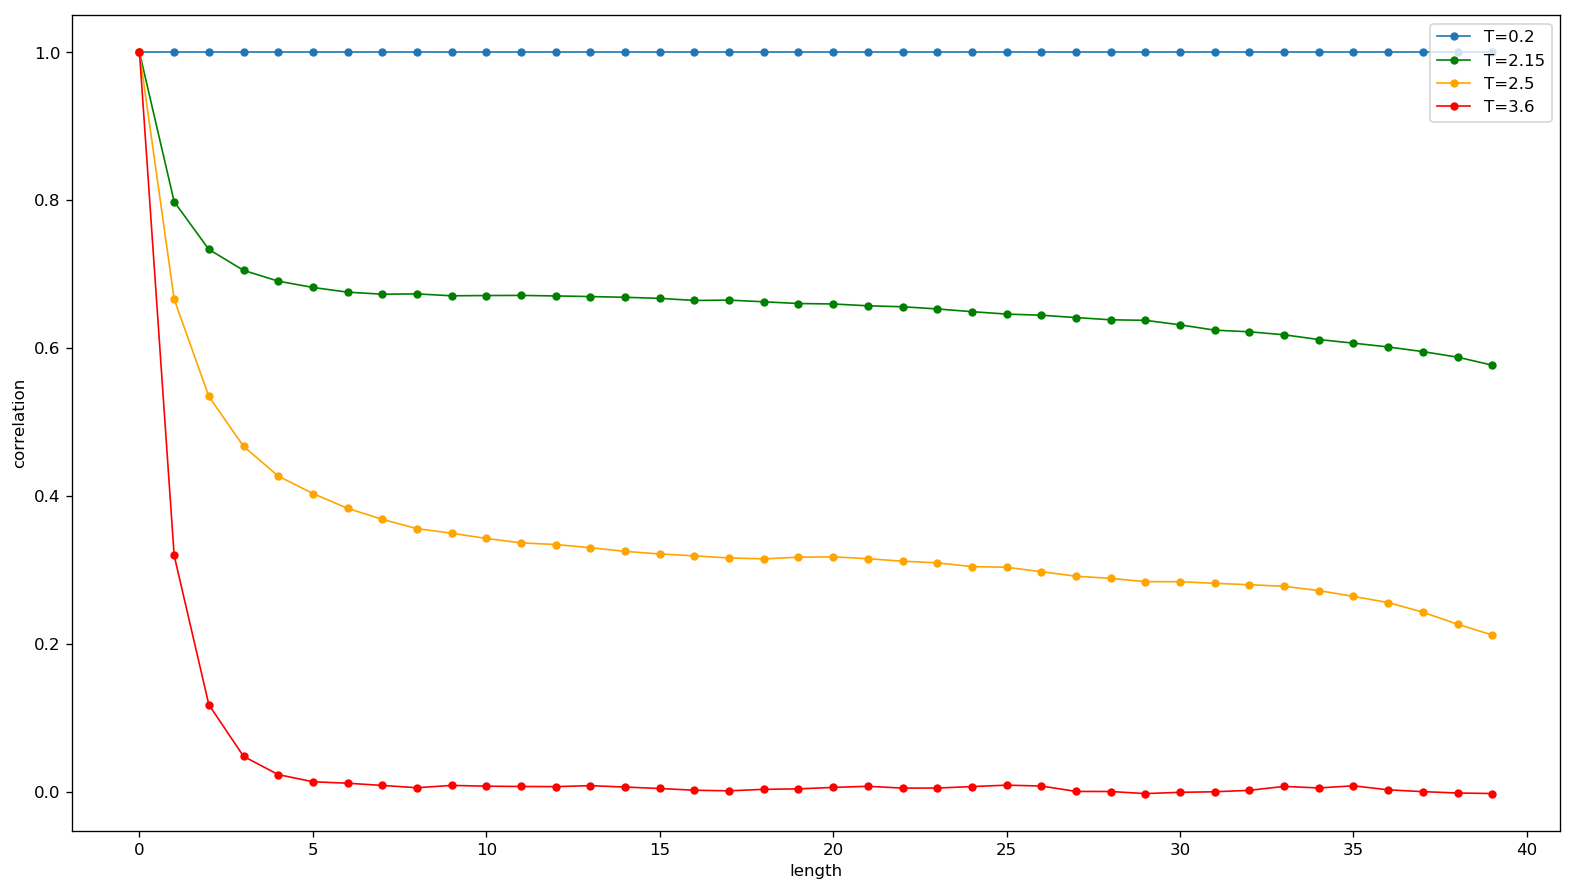
\includegraphics[scale=0.325]{cor.png}
\end{figure}

As to the correlation length $\xi$, from our analysis above we may suppose it to be monotonically decreasing with respect to the temperature $T$. Since performing logarithm operation to the data would introduce greater error, here we choose to obtain an estimation of $\xi$ by solving a squared error minimization problem via gradient decent method:
\begin{displaymath}
\hat\xi=argmin_\xi\ \ L(\xi) = \frac{1}{2}\sum_i(\hat\Gamma(r_i)-e^{-r/\xi})^2,
\  
\text{where }L'(\xi) = (e^{-r/\xi}-\hat\Gamma(r_i))\cdot e^{-r/\xi}\cdot \frac{r}{\xi ^2}
\end{displaymath}
. Our results are shown in the following image:
\begin{figure}[H]
\centering
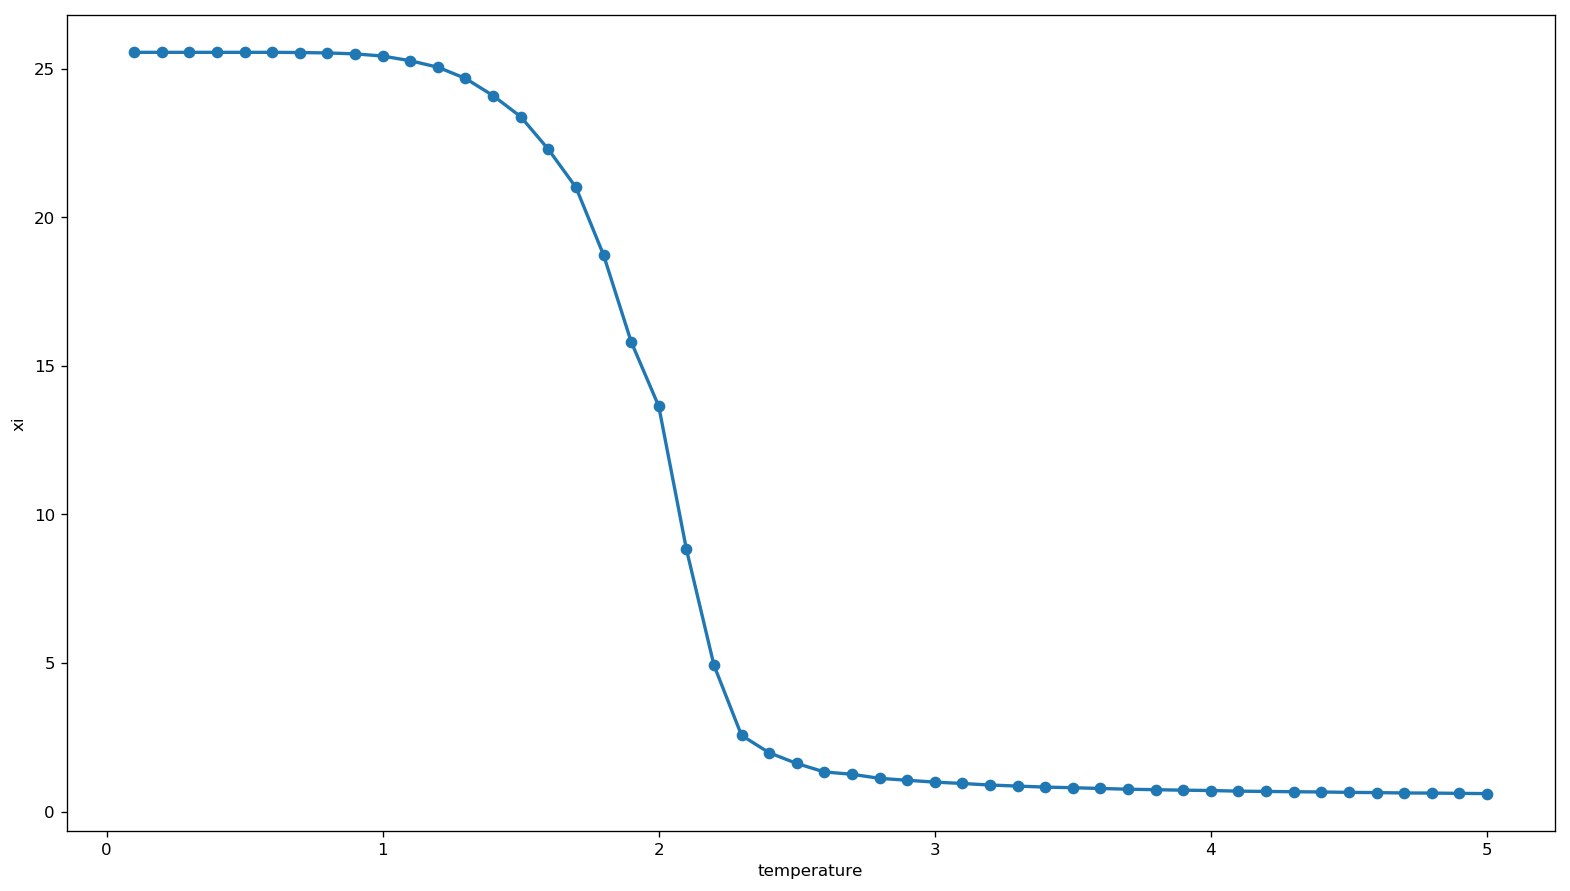
\includegraphics[scale=0.325]{xi.png}
\end{figure}
. The reason why the curve is flat when $T<1$ may be that the gradient decent method is only able to reach points within the ball centered at the initial value with radius $(N\times \text{step length})$ in N steps. So when $T < 1$, the $\hat\xi$ may not be the actual minimizer of $L$, but the maximal range the gradient decent method may reach in finite iterations. 

\subsection{Solution for part d)}
In part d) we would like to identify how $g_M$, $c_M$, $\xi$ should change with respect to $\epsilon=|1-\frac{T}{T^*}$ when $T$ is very close to $T^*$. We are informed these quantities may have quantitave relationships like:
\begin{displaymath}
\begin{aligned}
g_M &\sim m_0 \epsilon^a\\
c_M &\sim c_0 \epsilon^b\\
\xi &\sim \xi_0 \epsilon^c\\
\end{aligned}
\end{displaymath}
. However, our simulation results look like this:
\begin{figure}[H]
\centering
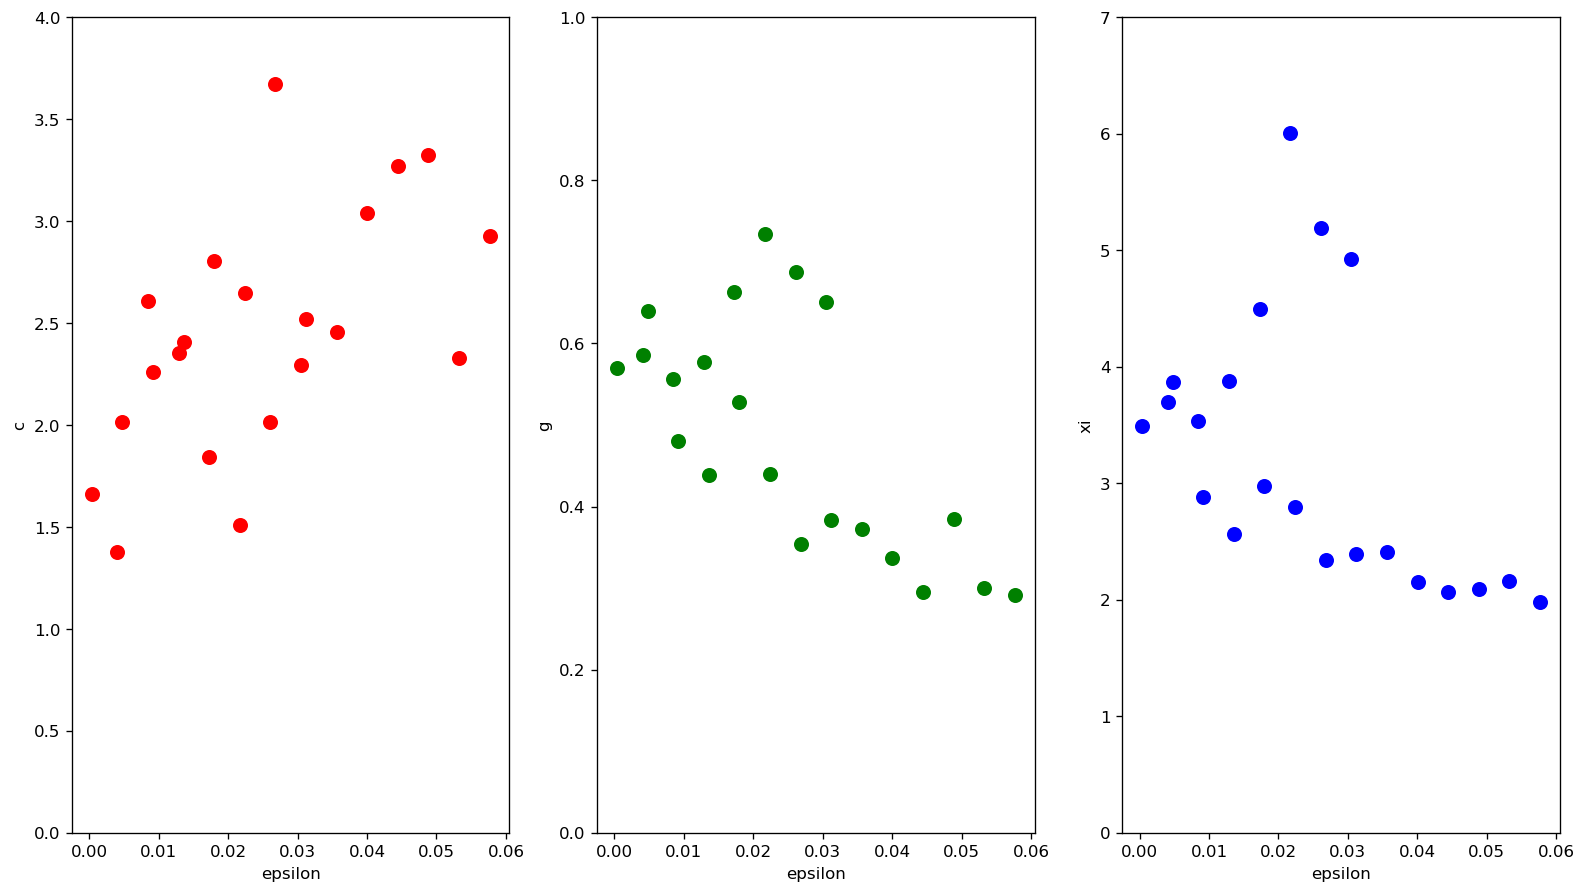
\includegraphics[scale=0.325]{eps.png}
\end{figure}
. And no special pattern can be recognized. We try to apply a series of techniques of parameter estimation but the results obtained make no sense. The reasons might be our simulations are not accurate enough, or the $\epsilon$ we take are not sufficiently small. 
\end{document}